\documentclass{rbfin}
\usepackage{amsmath}
\usepackage{amssymb} %mathbb
\usepackage{gensymb} % \degree
\usepackage{graphicx}
\usepackage{hyperref}

\begin{document}
\selectlanguage{brazil}
\shorttitle{Otimização Não Linear 2021} % appears on header every other page
\rbfe{}
\autor{Vinícius Claudino Ferraz, 2021}

\begin{center}
\Large

\textbf{Lista 3}

\normalsize

Matrícula $= 2019435823$
\end{center}

\large

\textbf{Questão 1.A}

\normalsize

\vspace{6mm}

\doublespacing

Ache o mínimo da função $f(x) = 0.65 - \cfrac{0.75}{1 + x^2} - 0.65 x \arctan \cfrac{1}{x}$ utilizando busca irrestrita com um tamanho de passo fixo de $0.1$ partindo do ponto $0.0$.

\singlespacing

\vspace{6mm}

\large

\textbf{Questão 1.B}

\normalsize

\vspace{6mm}

\doublespacing

Ache o mínimo da função $f(x)$ utilizando busca irrestrita com um tamanho de passo acelerado iniciando com um tamanho de $0.1$ partindo do ponto $0.0$.

\singlespacing

\vspace{6mm}

\large

\textbf{Questão 1.C}

\normalsize

\vspace{6mm}

\doublespacing

Ache o mínimo da função $f(x)$ utilizando busca exaustiva no intervalo $(0, 3)$ até atingir uma acurácia de $5\%$ do valor exato.

Dividimos em $n = 4$ pontos interiores: $v = (0.0, 0.6, 1.2, 1.8, 2.4, 3.0)$.

Calculamos $f$ em cada coordenada: $fv = (-0.1, -0.30331755, -0.19927290, -0.12019204, -0.07682089, -0.05241358)$.

A acurácia da segunda coordenada é $1 - \cfrac{0.30331755}{0.3100204} = 2.162067\%$.

Portanto, o mínimo ocorre em $x^* = 0.6$, $f(x^*) = -0.30331755$.

\singlespacing

\vspace{6mm}

\large

\textbf{Questão 1.D}

\normalsize

\vspace{6mm}

\doublespacing

Ache o mínimo da função $f(x)$ utilizando busca dicotômica no intervalo $(0, 3)$ até obter uma acurácia de $5\%$ do valor exato, com um $\delta = 0.0001$.

Inserimos $2$ pontos interiores: $v_1 = (0.0, 1.49995, 1.50005, 3.0)$.

Calculamos $f$ em cada coordenada: $fv_1 = (-0.1, -0.1540783, -0.1540652, -0.05241358)$.

O novo intervalo é $[0, 1.50005]$. Inserimos $2$ pontos interiores: $v_2 = (0, 0.749975, 0.750075, 1.50005)$.

Calculamos $f$ em cada coordenada: $fv_2 = (-0.1, -0.1540783, -0.1540652, -0.05241358)$.

O novo intervalo é $[0, 0.750075]$. No ponto médio, $f(0.3750375) = -0.3029708$.

A acurácia é $1 - \cfrac{0.3029708}{0.3100204} = 2.27391\%$.

Portanto, o mínimo ocorre em $x^* = 0.3750375$, $f(x^*) = -0.3029708$.

\singlespacing

\vspace{6mm}

\large

\textbf{Questão 1.E}

\normalsize

\vspace{6mm}

\doublespacing

Ache o mínimo da função $f(x)$ utilizando busca da bisseção no intervalo $(0, 3)$ até obter uma acurácia de $5\%$ do valor exato.

\singlespacing

\vspace{6mm}

\large

\textbf{Questão 2} 

\normalsize

\vspace{6mm}

\doublespacing

Faça o gráfico da função $f(x)$ no intervalo $(0, 3)$ e identifique o mínimo.

\begin{center}
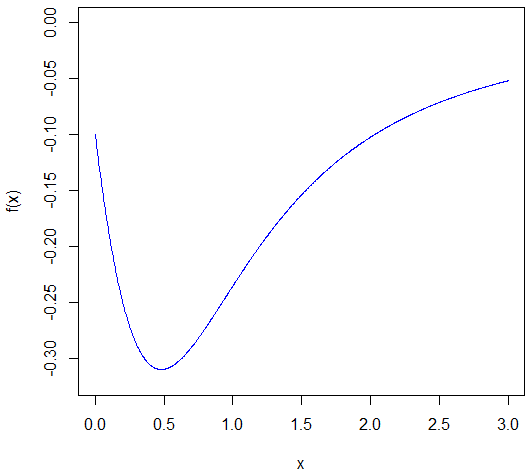
\includegraphics[scale=0.666]{q2}
\end{center}

O mínimo ocorre em $x^* = 0.4804805$, $f(x^*) = -0.3100204$.

\singlespacing

\vspace{6mm}

\large

\textbf{Questão 3.A}

\normalsize

\vspace{6mm}

\doublespacing

Ache o máximo da função $g(x) = \cfrac{0.5}{\sqrt{1 + x^2}} - \sqrt{1 + x^2} \left( 1 - \cfrac{0.5}{1 + x^2} \right) + x$ utilizando busca irrestrita com um tamanho de passo fixo de $0.1$ partindo do ponto $0.0$.

\singlespacing

\vspace{6mm}

\large

\textbf{Questão 3.B}

\normalsize

\vspace{6mm}

\doublespacing

Ache o máximo da função $g(x)$ utilizando busca irrestrita com um tamanho de passo acelerado iniciando com um tamanho de $0.1$ partindo do ponto $0.0$.

\singlespacing

\vspace{6mm}

\large

\textbf{Questão 3.C}

\normalsize

\vspace{6mm}

\doublespacing

Ache o máximo da função $g(x)$ utilizando busca exaustiva no intervalo $(0, 3)$ até atingir uma acurácia de $5\%$ do valor exato.

Pelo método do gráfico (questão $2$), o máximo exato ocorre em $x^* = 0.7867868$, $g(x^*) = 0.300283$.

Dividimos em $n = 3$ pontos interiores: $v = (0.00, 0.75, 1.50, 2.25, 3.00)$.

Calculamos $g$ em cada coordenada: $gv = (0, 0.3, 0.2519246, 0.1939240, 0.1539501)$.

A acurácia da segunda coordenada é $1 - \cfrac{0.3}{0.300283} = 0.09424443\%$.

Portanto, o máximo ocorre em $x^* = 0.75$, $g(x^*) = 0.3$.

\singlespacing

\vspace{6mm}

\large

\textbf{Questão 3.D}

\normalsize

\vspace{6mm}

\doublespacing

Ache o máximo da função $g(x)$ utilizando busca dicotômica no intervalo $(0, 3)$ até obter uma acurácia de $5\%$ do valor exato, com um $\delta = 0.0001$.

Inserimos $2$ pontos interiores: $v = (0.0, 1.49995, 1.50005, 3.0)$.

Calculamos $g$ em cada coordenada: $gv = (0, 0.251929, 0.2519202, 0.1539501)$.

O novo intervalo é $[0, 1.50005]$. No ponto médio, $g(0.750025) = 0.3000004$.

A acurácia é $1 - \cfrac{0.3000004}{0.300283} = 0.09411127\%$.

Portanto, o máximo ocorre em $x^* = 0.750025$, $g(x^*) = 0.3000004$.

\singlespacing

\vspace{6mm}

\large

\textbf{Questão 3.E}

\normalsize

\vspace{6mm}

\doublespacing

Ache o máximo da função $g(x)$ utilizando busca da bisseção no intervalo $(0, 3)$ até obter uma acurácia de $5\%$ do valor exato.

\singlespacing

\vspace{6mm}

\large

\textbf{Questão 4.A}

\normalsize

\vspace{6mm}

\doublespacing

Encontre o máximo da função $g(x)$ utilizando método de Fibonacci com $n = 8$.

\singlespacing

\vspace{6mm}

\large

\textbf{Questão 4.B}

\normalsize

\vspace{6mm}

\doublespacing

Encontre o máximo da função $g(x)$ utilizando método da Seção Áurea com $n = 8$.

\singlespacing

\vspace{6mm}

\large

\textbf{Questão 5}

\normalsize

\vspace{6mm}

\doublespacing

Faça o gráfico de contorno para a função $p(x_1, x_2) = (x_1 + 2x_2 - 7)^2 +(2x_1 + x_2 - 5)^2$ na região $(-5 \le x_1 \le 5$, $-3 \le x_2 \le 6)$ e identifique o ponto ótimo.

\begin{center}
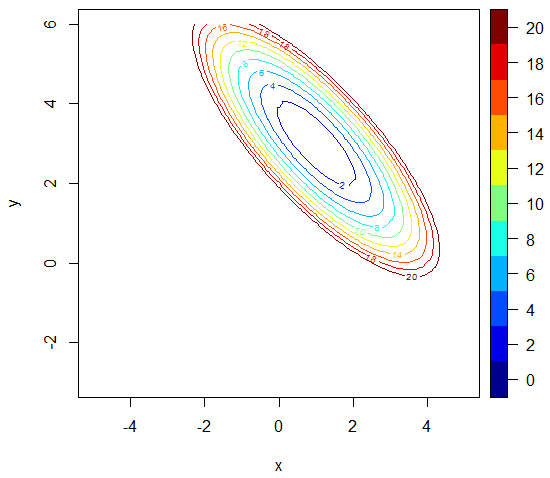
\includegraphics[scale=0.666]{q5}
\end{center}

O mínimo ocorre em $x^* = (1,3)$, $p(x^*) = 0$.

\singlespacing

\vspace{6mm}

\large

\textbf{Questão 6}

\normalsize

\vspace{6mm}

\doublespacing

Faça o gráfico de contorno para a função $q(x_1, x_2) = 2(x_2 - x_1^2)^2 +(1 - x_1)^2$ na região $(-4 \le x_1 \le 4, -3 \le x_2 \le 6)$ e identifique o ponto ótimo.

\begin{center}
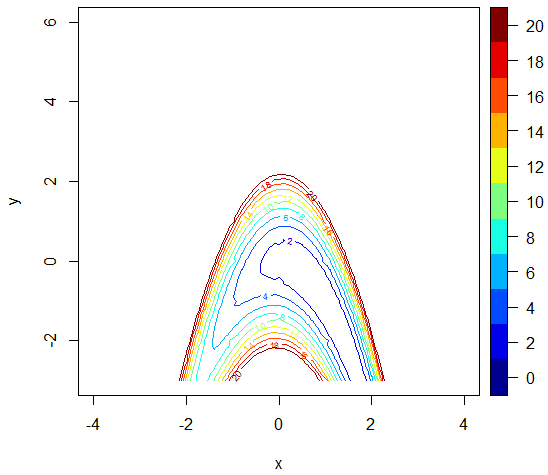
\includegraphics[scale=0.666]{q6}
\end{center}

O mínimo ocorre em $x^* = (1,-1)$, $q(x^*) = 0$.

\singlespacing

\vspace{6mm}

\large

\textbf{Questão 7}

\normalsize

\vspace{6mm}

\doublespacing

Realize duas iterações do Método de Newton para minimizar a função $h(x, y) = 100(y - x^2)^2 +(1 - x)^2$ com um $(x_0, y_0) = (-1.2, 1.0)$.

$\nabla h(x,y) = (-400x(y - x^2) - 2(1 - x), 200(y - x^2))$

$\nabla h(-1.2, 1.0) = (-215.6,-88)$

$H(x,y) = \begin{pmatrix} -400(y - 3x^2) + 2 & -400x  \\ -400x & 200 \end{pmatrix}$

$H(-1.2, 1.0) = \begin{pmatrix} 1330 & 480 \\ 480 & 200 \end{pmatrix} = H_1$

$(x_1, y_1) = (-1.2, 1.0) - H_1^{-1} \cdot (-215.6,-88) = (-1.175281, 1.380674)$

$\nabla h(-1.175281, 1.380674) = (-4.6378164,-0.1222068)$

$H(-1.175281, 1.380674) = \begin{pmatrix} 1107.2726 & 470.1124 \\ 470.1124 & 200 \end{pmatrix} = H_2$

$(x_2, y_2) = (-1.175281, 1.380674) - H_2^{-1} \cdot (-4.6378164,-0.1222068) = (0.7631149, -3.175034)$ ; $h(x_2, y_2) = 1411.845$.

Péssimo. Mas, continuando, o mínimo ocorre em $(x_3, y_3) = (0.7634297, 0.5828248)$ ; $h(x_3, y_3) = 0.05596552$.

\singlespacing

\vspace{6mm}

\large

\textbf{Questão 8}

\normalsize

\vspace{6mm}

\doublespacing

Compare os gradientes da função $h(x, y)$ em $(x_0, y_0) = (0.5, 0.5)$ obtidos utilizando os seguintes métodos:

a) Resolução analítica:

$\nabla h(x,y) = (-400x(y - x^2) - 2(1 - x), 200(y - x^2))$

$v_1 = \nabla h(0.5, 0.5) = (-51,50) = (p_1, q_1)$

b) Método da diferença centrada:

Sejam $\Delta x = \Delta y = 0.0001$.

$p_2 = \cfrac{\partial h}{\partial x} = \cfrac{h(x + \Delta x,y) - h(x - \Delta x,y)}{2\Delta x} = \cfrac{h(0.5001,0.5) - h(0.4999,0.5)}{0.0001}$

$q_2 = \cfrac{\partial h}{\partial y} = \cfrac{h(x,y + \Delta y) - h(x,y - \Delta y)}{2\Delta y} = \cfrac{h(0.5,0.5001) - h(0.5,0.4999)}{0.0001}$

$v_2 = (p_2, q_2) = (-51,50)$.

c) Método da diferença progressiva:

$p_3 = \cfrac{\partial h}{\partial x} = \cfrac{h(x + \Delta x,y) - h(x,y)}{\Delta x} = \cfrac{h(0.5001,0.5) - h(0.5,0.5)}{0.0001}$

$q_3 = \cfrac{\partial h}{\partial y} = \cfrac{h(x,y + \Delta y) - h(x,y)}{\Delta y} = \cfrac{h(0.5,0.5001) - h(0.5,0.5)}{0.0001}$

$v_3 = (p_3, q_3) = (-50.9949, 50.0100)$.

d) Método da diferença regressiva:

$p_4 = \cfrac{\partial h}{\partial x} = \cfrac{h(x,y) - h(x - \Delta x,y)}{\Delta x} = \cfrac{h(0.5,0.5) - h(0.4999,0.5)}{0.0001}$

$q_4 = \cfrac{\partial h}{\partial y} = \cfrac{h(x,y) - h(x,y - \Delta y)}{\Delta y} = \cfrac{h(0.5,0.5) - h(0.5,0.4999)}{0.0001}$

$v_4 = (p_4, q_4) = (-51.0051, 49.9900)$.

e) Comparação:

$v_2 = v_1$ ; $p_3 > p_1$ ; $q_3 > q_1$ ; $p_4 < p_1$ ; $q_4 < q_1$.

$\vert p_3 - p_1 \vert = 0.0051 = \vert p_4 - p_1 \vert$ ; $\cfrac{0.0051}{51} = 0.01\%$ de erro.

$\vert q_3 - q_1 \vert = 0.01 = \vert q_4 - q_1 \vert$ ; $\cfrac{0.01}{50} = 0.02\%$ de erro.

\singlespacing

\vspace{6mm}

\large

\textbf{Questão 9}

\normalsize

\vspace{6mm}

\doublespacing

Realize duas iterações do Método de Newton para minimizar a função $\varphi(x, y) = 2 x^2 + y^2$ com um $(x_0, y_0) = (1, 2)$.

$\nabla \varphi(x,y) = (4x, 2y)$

$\nabla \varphi(1, 2) = (4, 4)$

$H = \begin{pmatrix} 4 & 0 \\ 0 & 2 \end{pmatrix} \Rightarrow H^{-1} = \begin{pmatrix} 0.25 & 0 \\ 0 & 0.5 \end{pmatrix}$

$(x_1, y_1) = (1, 2) - \begin{pmatrix} 0.25 & 0 \\ 0 & 0.5 \end{pmatrix} \cdot (4, 4) = (0 , 0)$

$\nabla \varphi(0, 0) = (0, 0)$

O mínimo ocorre em $(x_2, y_2) = (0, 0) - \begin{pmatrix} 0.25 & 0 \\ 0 & 0.5 \end{pmatrix} \cdot (0, 0) = (0, 0)$ ; $\varphi(x_2, y_2) = 0$.

\singlespacing

\vspace{6mm}

\large

\textbf{Questão 10}

\normalsize

\vspace{6mm}

\doublespacing

Realize duas iterações do Método de Newton para minimizar a função $\psi(x, y, z) = x^2 + 3 y^2 + 6 z^2$ com um 

$(x_0, y_0, z_0) = (2, -1, 1)$.

$\nabla \psi(x,y,z) = (2x, 6y, 12z)$

$\nabla \psi(2, -1, 1) = (4, -6, 12)$

$H = \begin{pmatrix} 2 & 0 & 0 \\ 0 & 6 & 0 \\ 0 & 0 & 12 \end{pmatrix} \Rightarrow H^{-1} = \begin{pmatrix} 0.5 & 0 & 0 \\ 0 & 1/6 & 0 \\ 0 & 0 & 1/12 \end{pmatrix}$

$(x_1, y_1, z_1) = (2, -1, 1) - \begin{pmatrix} 0.5 & 0 & 0 \\ 0 & 1/6 & 0 \\ 0 & 0 & 1/12 \end{pmatrix} \cdot (4, -6, 12) = (0 , 0, 0)$

$\nabla \psi(0, 0, 0) = (0, 0, 0)$

O mínimo ocorre em $(x_2, y_2, z_2) = (0, 0, 0) - \begin{pmatrix} 0.5 & 0 & 0 \\ 0 & 1/6 & 0 \\ 0 & 0 & 1/12 \end{pmatrix} \cdot (0, 0, 0) = (0, 0, 0)$ ; $\psi(x_2, y_2, z_2) = 0$.

\singlespacing

\vspace{6mm}

Versão de 10/janeiro/2022\footnote{Fora da caridade não há salvação.} por Vinicius Claudino Ferraz.

\end{document}
